\section{Introduction}
\label{sec:intro}
 In the era of Big Data, visualization arises as an important mean to explore and derive insights from data.  However, visualized information such as relationships and trends may emerge from random noise.  Without proper statistical control, users may mistake visually significant observations as statistically significant.  Worse yet, systems that search and recommend visualized information would produce large number of questionable insights.  
A recent study shows that visualization and recommendation without considering the risk of false discovery, such as Vizdom~\cite{vizdom}, SeeDB~\cite{seedb} and Data Polygamy~\cite{polygamy}, becomes unusable on datasets with any randomness \cite{binnig2017sustainable}.

False discovery due to random noise is pervasive in visual data exploration on real-world datasets. For example, when using Vizdom~\cite{vizdom} to explore a recently conducted survey on personal habits and opinions~\cite{binnig2017sustainable}, we observed that the preference on watching films on DVD produced visually different proportion of belief in aliens, as shown in Figure~\ref{fig:example}A and B.  But such predictor proved neither much sensible nor statistically significant.  More alarmingly, more and more such observation-based hypotheses may be formulated as the user continues to explore the dataset, and hence quickly increase the expected number of false discoveries. For an example of the same survey, after searching through a few different comparisons, we stumbled upon a visualization that suggests hair color predicts whether one knows about Michael Stonebraker, and it would be statistically significant if considered as a lone hypothesis. This phenomenon is often referred to as data dredging or $p$-hacking~\cite{head2015extent}, and formally known as the multiple comparison problem~\cite{shaffer1995multiple}.

Several challenges exist to control the false discoveries in interactive data exploration.  To begin with, most statisticians evaluate hypotheses in a passive computing environment such as R~\cite{R}; whereas in visual data exploration, the system also needs to assist the user in the hypothesis formulation and the hypothesis test selection. Secondly, interactive data exploration generates hypotheses dynamically to follow the process of human decision making.  However the traditional statistical procedures such as Bonferroni~\cite{bonferroni1936teoria} and Sequential FDR~\cite{g2016sequential} are not dynamic in that they require knowing all the hypotheses a priori before finalizing the inference on statistical significance.  Moreover, these traditional techniques assume complete pass of the data, and hence would make the system non-interactive on larger datasets.  But progressive computation proves to be an alternative paradigm more appealing for interactive visualization on Big Data~\cite{zgraggen2016progressive, onlineagg, vizdom}.  Finally, data exploration can also be automated as in visualization search and recommendation. The algorithms used in this automatic data exploration should also be subject to false discovery control.

Thus, we implemented the recent advance in interactive false discovery control that is both dynamic and progressive, and applied to both manual and automatic data exploration~\cite{zhao2016controlling}. Our system \system{} is based on Vizdom~\cite{vizdom} and addresses the aforementioned challenges, namely,
\begin{itemize}
    \item To formulate hypotheses via user interaction;
    \item To visualize the statistical significance and other contextual information for each observation;
    \item To control multiple hypotheses dynamically during data exploration;
    \item To progressively compute the risk of false discovery on larger data.
\end{itemize}

\begin{figure}
\centering
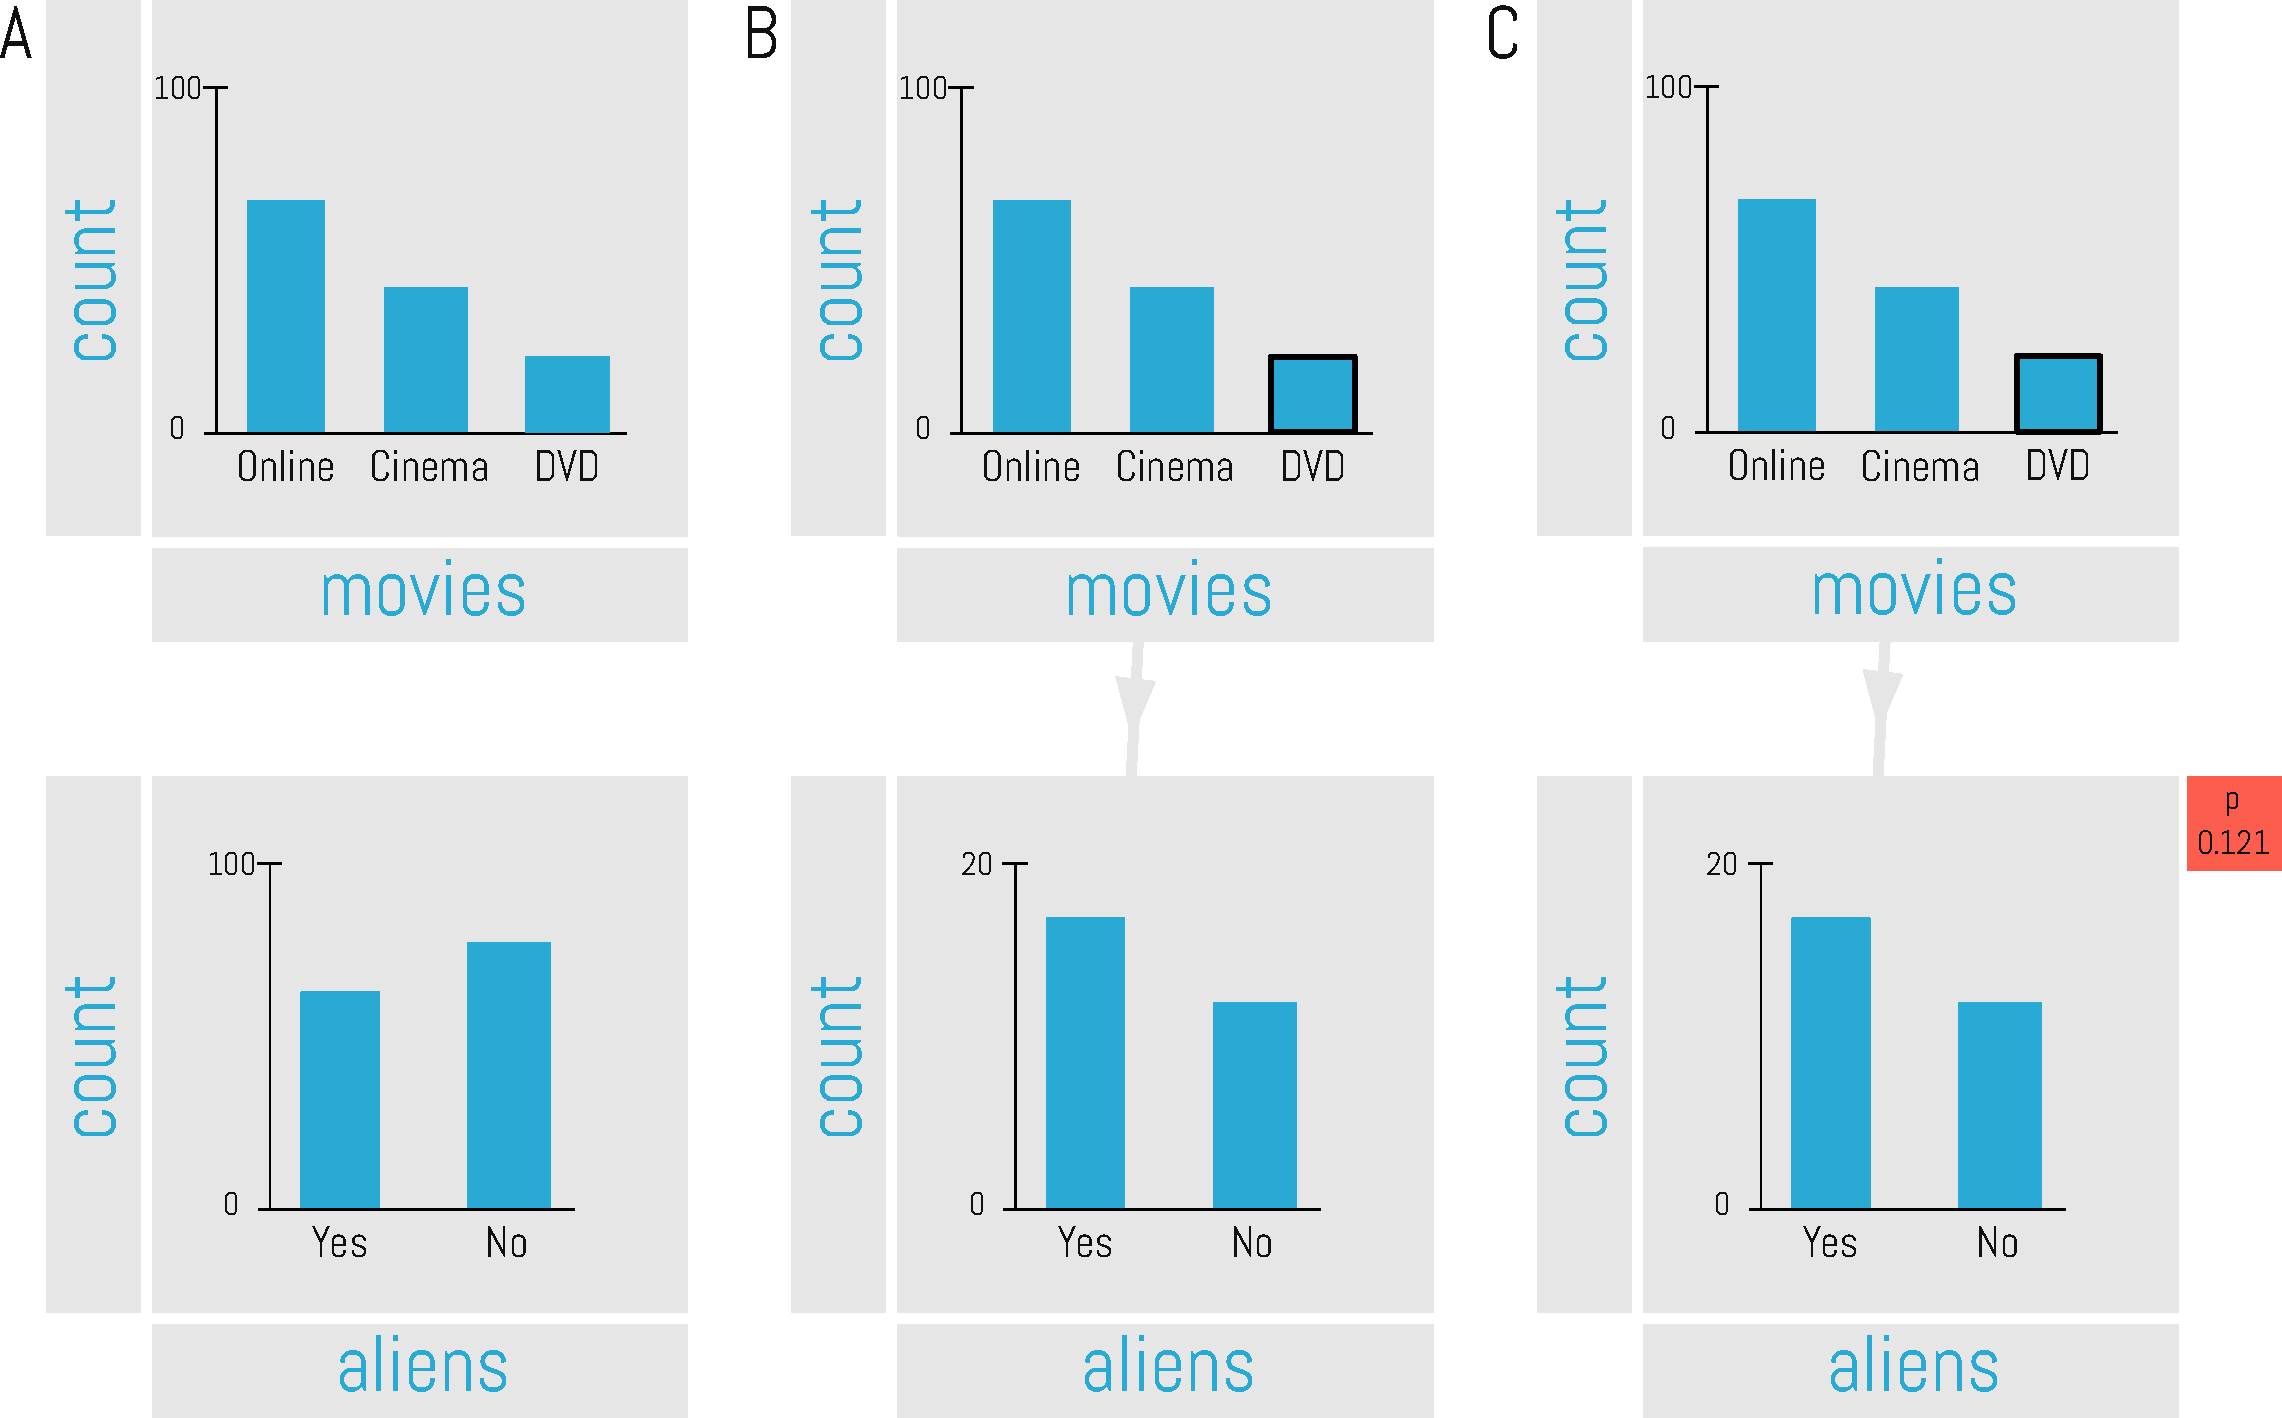
\includegraphics[width=0.48\textwidth]{figures/example}
\caption{Example of a visualization network where users might be led to false discoveries without automaitc hypothesis generation. }
\label{fig:example}	
\end{figure}